\documentclass[border=10pt]{standalone}
\usepackage{pgfplots}
\usepgfplotslibrary{colormaps}
\pgfplotsset{compat=1.18}

\begin{document}
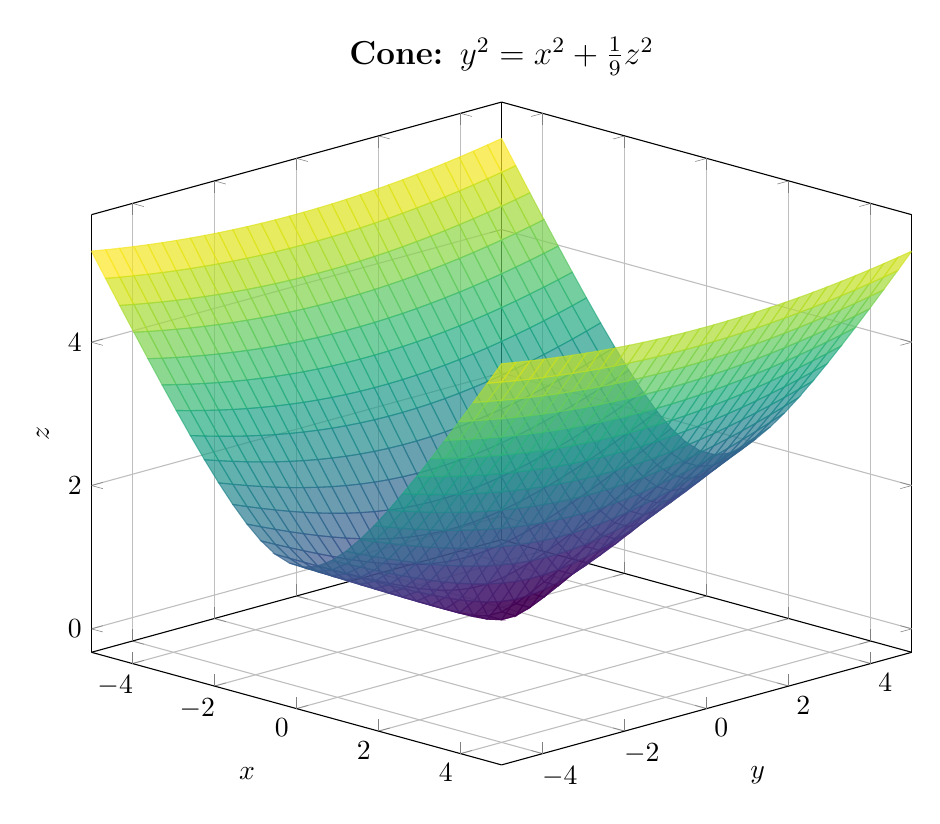
\begin{tikzpicture}
\begin{axis}[
    view={45}{20},
    xlabel={$x$},
    ylabel={$y$},
    zlabel={$z$},
    title={Cone: $y^2 = x^2 + \frac{1}{9}z^2$},
    xlabel style={font=\bfseries},
    ylabel style={font=\bfseries},
    zlabel style={font=\bfseries},
    title style={font=\bfseries\large},
    colormap/viridis,
    grid=major,
    width=12cm,
    height=10cm
]
% Positive nappe: y = sqrt(x^2 + z^2/9)
\addplot3[surf, shader=flat corner, samples=30, opacity=0.7] 
    {sqrt(x^2 + y^2/9)};
\end{axis}
\end{tikzpicture}
\end{document}